
\documentclass[border=10pt]{standalone}
\usepackage{pgfplots}
\pgfplotsset{compat=1.18}
\begin{document}
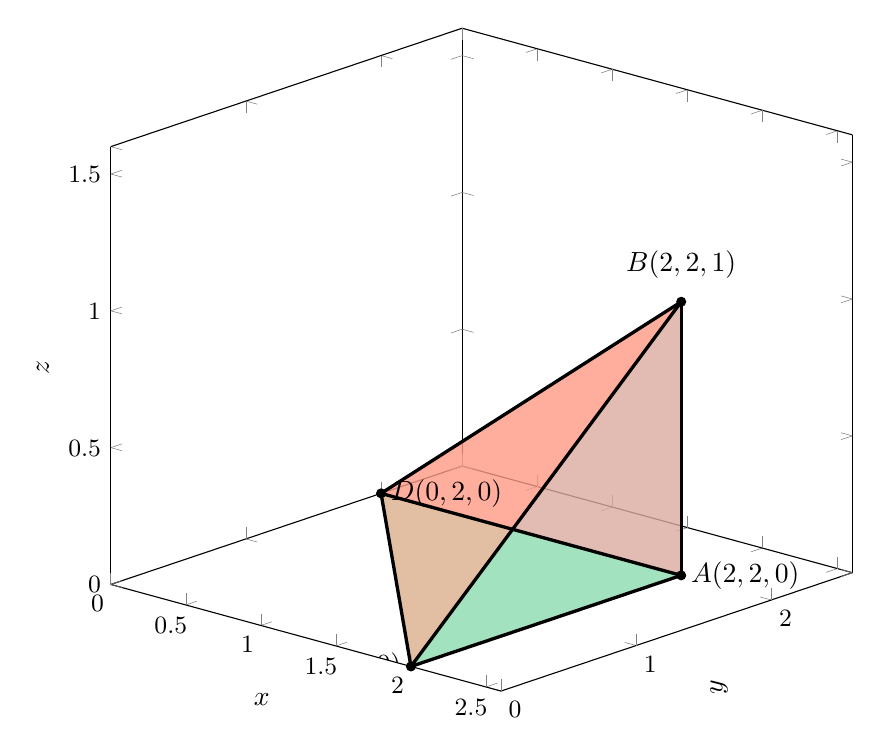
\begin{tikzpicture}
\begin{axis}[
    view={42}{20},
    xlabel={$x$}, ylabel={$y$}, zlabel={$z$},
    xmin=0, xmax=2.6, ymin=0, ymax=2.6, zmin=0, zmax=1.6,
    width=11cm, height=10cm,
    axis lines=box,
    tick label style={font=\small},
]
% ---- faces (filled triangles) ----
\addplot3[fill=blue!45,draw=none,opacity=0.55] coordinates {(2,2,0) (2,2,1) (2,0,0) (2,2,0)};
\addplot3[fill=orange!55,draw=none,opacity=0.55] coordinates {(2,2,0) (2,2,1) (0,2,0) (2,2,0)};
\addplot3[fill=green!45,draw=none,opacity=0.55] coordinates {(2,2,0) (2,0,0) (0,2,0) (2,2,0)};
\addplot3[fill=red!45,draw=none,opacity=0.55] coordinates {(2,2,1) (2,0,0) (0,2,0) (2,2,1)};
% ---- edges ----
\addplot3[black,very thick] coordinates {(2,2,0) (2,2,1)};
\addplot3[black,very thick] coordinates {(2,2,0) (2,0,0)};
\addplot3[black,very thick] coordinates {(2,2,0) (0,2,0)};
\addplot3[black,very thick] coordinates {(2,2,1) (2,0,0)};
\addplot3[black,very thick] coordinates {(2,2,1) (0,2,0)};
\addplot3[black,very thick] coordinates {(2,0,0) (0,2,0)};
% ---- vertices ----
\addplot3[only marks,mark=*,mark size=1.6pt,black] coordinates {(2,2,0) (2,2,1) (2,0,0) (0,2,0)};
\node[anchor=south] at (axis cs:2,2,1.05) {$B(2,2,1)$};
\node[anchor=west]  at (axis cs:2,2,0)  {$A(2,2,0)$};
\node[anchor=east]  at (axis cs:2,0,0)  {$C(2,0,0)$};
\node[anchor=west]  at (axis cs:0,2,0)  {$D(0,2,0)$};
\end{axis}
\end{tikzpicture}
\end{document}
